% This is samplepaper.tex, a sample chapter demonstrating the
% LLNCS macro package for Springer Computer Science proceedings;
% Version 2.20 of 2017/10/04
%
\documentclass[runningheads]{llncs}
%
\usepackage{graphicx}
\usepackage[utf8x]{inputenc}
\usepackage[ampersand]{easylist}
\usepackage{graphicx}
% Used for displaying a sample figure. If possible, figure files should
% be included in EPS format.
%
% If you use the hyperref package, please uncomment the following line
% to display URLs in blue roman font according to Springer's eBook style:
% \renewcommand\UrlFont{\color{blue}\rmfamily}

\begin{document}
%
\title{Conversation-Based Complex Event Management in Smart-Spaces}
%\title{Exploring Complex Event Management
%in Smart-Spaces through a
%Conversation-Based Approach}
%
\titlerunning{Conversation-Based Complex Event Management in Smart-Spaces}
% If the paper title is too long for the running head, you can set
% an abbreviated paper title here
%
\author{André Sousa Lago\inst{1}\orcidID{0000-0002-4534-9180} \and
Hugo Sereno Ferreira\inst{2}\orcidID{0000-0002-4963-3525}}
% \author{First Author\inst{1}\orcidID{0000-1111-2222-3333} \and
% Second Author\inst{2,3}\orcidID{1111-2222-3333-4444} \and
% Third Author\inst{3}\orcidID{2222--3333-4444-5555}}
%
\authorrunning{André S. Lago, Hugo S. Ferreira}
% First names are abbreviated in the running head.
% If there are more than two authors, 'et al.' is used.
%
\institute{Faculty of Engineering of University of Porto, 4200-465 Porto, Portugal \and
Department of Informatics Engineering, Faculty of Engineering of University of Porto, 4200-465 Porto, Portugal}
%
\maketitle              % typeset the header of the contribution
%
\begin{abstract}
    Smart space management can be done in many ways. On one hand, there are conversational assistants such as the Google Assistant or Amazon Alexa that enable users to comfortably interact with smart spaces with only their voice, but these have limited functionality and are usually limited to simple commands. On the other hand, there are visual interfaces such as IBM's Node-RED that enable complex features and dependencies between different devices. However, these are limited since they require users to have a technical knowledge of how the smart devices work and the system's interface is more complicated and harder to use since they require a computer.
    This project proposes a new conversational assistant - Jarvis - that combines the ease of use of current assistants with the operational complexity of the visual platforms. The goal of Jarvis is to make it easier to manage smart spaces by providing intuitive commands and useful features. Jarvis integrates with already existing user interfaces such as the Google Assistant, Slack or Facebook Messenger, making it very easy to integrate with existing systems. Jarvis also provides an innovative feature - causality queries - that enable users to ask it why something happened. For example, a user can ask "\textit{why did the light turn on?}" to understand how the system works.

\keywords{Human-centered computing → Natural language interfaces.}
\end{abstract}
%
%
%
\section{Introduction}

\subsection{Internet of Things}

The Internet of Things, or IoT, is the networked connection of everyday objects, which is often equipped with a collective sense of intelligence~\cite{Xia2012}. The integration of such objects creates a huge range of distributed systems that are able to interact with the environment and human beings around them in a lot of different ways.

The flexibility of IoT systems has enabled their use across many different product areas and markets, including smart homes, smart cities, healthcare, transportation, retail, wearables, agriculture and industry~\cite{Rahul2017}.

IoT is a booming technological market, and Gartner predicts that 11.2 billion devices will be connected in 2018, a number that is also predicted to almost double over the following 2 years, becoming 20.4 billion devices by 2020~\cite{VanderMeulen2017}. The Boston Consulting Group also estimates that by 2020 companies will spend 250 billion Euros in IoT on top of what they already spend on other technologies~\cite{Hunke2017}. This means that not only more people will be using IoT, but also that it will be present in a lot of different environments and situations. This represents a unique opportunity for IoT to evolve as a facilitator on people’s lives. After all, having intelligently connected devices around us should help us make our day to day lives easier.

This boom in worldwide connected devices has led to a lot of different applications of these technologies across countries and product areas. Although being a relatively small sample, the examples below demonstrate different use cases of IoT when combined with multiple technologies and markets~\cite{Chen2014,Lee2015,Xu2014}.

\textbf{Smart Homes} are the IoT application of domotics. While domotics usually refers to individual systems that perform isolated tasks automatically, smart homes usually refer to a set of connected sensors and electronics that allow for a house to be more autonomous. Some smart houses include appliances such as fridges that remind users when a certain item is about to run out, self-regulating temperature systems or self-locking door and window mechanisms. Perhaps more importantly, many of these devices can be controlled or monitored remotely which provides users with a greater sense of control of their appliances.

\textbf{Wearables} are devices that are worn like clothes, accompanying human beings in their regular activities. Some examples of wearable devices are smartwatches, step counters or smart glasses. With the sizes of processors and electronic boards shrinking, the capabilities of these devices have increased, and such can be seen in the growth of this industry segment which was predicted to surpass 4 billion dollars in 2017 by Forbes~\cite{Marr2016}.

\textbf{Smart Cities} are a concept similar to smart homes, where the same technology is applied in the context of a public space. These usually aim towards simplifying urban life, or making it more environment-friendly. The most common use cases in this segment are smart parking spaces, smart waste management systems or smart street lighting.

\textbf{Retail} can also be an interesting use case for IoT as it can benefit both customers and store managers. In these cases, IoT can not only help customers instantly know whether a certain product is in stock or not, but also help the manager determine when to order a certain product based on its current shelf stock.

\textbf{Healthcare} is yet another field where IoT can be very beneficial, as it can help doctors remotely keep track of a patient’s live status, or receive an alert when a problem is detected with a patient. An article by IBM even alerts that even though there are a lot of problems around IoT in healthcare, especially due to data privacy, it can help reduce healthcare costs or improve the outcome of treatments~\cite{Patel2017}.

Finally, \textbf{customized smart spaces} are a logical consequence of the growth of IoT and its associated products, as it became possible for almost everyone to create a customized IoT experience based on products and hardware available. In any IoT system, the essential items are the physical devices that are connected by the system and interact with the environment. In this document these are called \textbf{leaf devices}. 

The first step to create a customized smart space is to acquire the leaf devices, depending on the intended use for the system. Some of the most common leaf devices are temperature sensors, motion sensors and remote light switches. Although some of these devices have controllers of their own that can be programmed or controlled in a certain way, it is also possible to acquire \textbf{middleware devices} that connect to the leaf devices, and therefore are able to read and modify their current status. 

Arduino boards and Raspberry Pi computers are often used as middleware devices due to their setup simplicity and low cost. For example, a Raspberry Pi’s GPIO\footnote{General Purpose Input/Output, multi-purpose ports that can be programmed for different inputs and outputs} ports can be simultaneously connected to a luminosity sensor and a light switch. That way, not only the luminosity value of the sensor can be sent to a remote server via Wi-Fi, but also the light switch can be turned on when the luminosity drops below a certain level. Arduino boards can also be used to increase the capacity of simpler devices such as sensors or actuators. For example, an Arduino board can be connected to a sensor providing it with a connection to a local network, so that the sensor’s status can be accessed remotely.

Once the devices are acquired, it is necessary to connect them to a network and manage their behavior. To achieve this, a common technique is to use a \textbf{supervisor device}, a middleware device that acts as a supervisor for all the other devices. A computer or Raspberry Pi are common supervisor devices as these usually require a bit more power than alternatives like Arduino boards can offer. Once the supervisor device is ready, platforms like Node-RED\footnote{\url{https://nodered.org/}} or Home Assistant\footnote{\url{https://home-assistant.io/}} can be installed to facilitate the management of the system as a whole. These \textbf{management platforms} are described thoroughly below.

As a practical example, let’s picture a user that wants to have a luminosity sensor and a temperature sensor in his room, and an actuator that can open and close the window. With these, the user wants to have a dashboard where he can consult the history of the room’s luminosity as well as the status (open/closed) of the window. Finally, the user wants the window to be shut if the temperature drops below a certain level. To achieve this functionality, all the user needs is to buy the actual sensors, the actuator and a Raspberry Pi. Then, the sensors and the actuator are connected to the Pi, which is then given an installation of Node-RED, so that the user can make the window close when the temperature drops.

\subsection{Visual Programming Paltforms}

Visual programing platforms, or VPPs, are tools that are usually installed in supervisor devices in IoT systems so that they can access all the devices and components in such systems. Because of that, these platforms can offer users with extensive and friendly UIs through which the user can visualize the state of the system, customize its behavior or even configure the system’s devices themselves. Some VPPs even offer integrations with third parties such as Twitter or Instagram, so that their APIs can be used as part of the system’s behavioral rules.

As an example, we will take a look at one of the most popular VPPs (Node-RED), but it is important to note that there are other relevant alternatives, such as the Home Assistant\footnote{\url{https://home-assistant.io/}}.

\textbf{Node-RED}\footnote{\url{https://nodered.org/}} is a tool developed by IBM’s Emerging Technology Services team in 2013, and is now a part of the JS Foundation. Node-RED follows a flow-based programming approach to the management of an IoT system, providing its users with a Node.js-based web application through which they can create, edit and delete system rules and connections in an interface that displays rules and connections as a flow of information, events or actions.

In Node-RED, system devices are represented as colourful nodes that possess specific properties and actions which can be interconnected with other nodes. Similarly, conditions, actions and events are also represented as nodes, which makes it easy to understand how elements can be connected in the platform. Being based in Node.js, all that is required to use Node-RED is to have it running in a supervisor device in the system, such as a Raspberry Pi, and then the platform can be accessed through any regular web browser.

\begin{figure}
    \begin{center}
        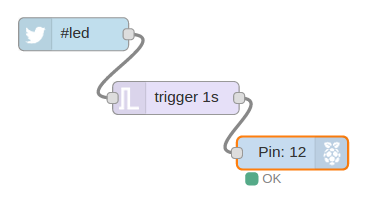
\includegraphics[width=0.5\textwidth]{figures/nodered-simple.jpg}
        \caption{Simple setup of a Node-RED managed system.} \label{fig:nodered-simple}
    \end{center}
\end{figure}

Figure~\ref{fig:nodered-simple} represents a simple application of Node-RED to manage an IoT system. In the example, the user has defined a flow where built-in Node-RED nodes are connected in a flow of information. With blocks similar to those displayed by the figure it is possible to not only send commands to IoT devices but also act upon events received from them, which brings the possibility to create rather complex systems with many dependency rules.

When multiple rules such as the one displayed in Figure~\ref{fig:nodered-simple} are setup in Node-RED, it becomes possible to create complex systems that turn on lights at a certain time, activate devices such as microwave ovens when it is time for breakfast or close the windows if it starts raining.

VPPs can be extremely useful for users of custom smart spaces due to the flexibility and power they provide. However, they possess several disadvantages that make them somewhat hard to use, especially for users that are not entirely comfortable with understanding how certain technologies work.

Let's imagine a Node-RED system, embedded in a user’s home, with multiple devices. Even if there are only a couple of dozens of rules defined, it can be extremely difficult to understand why a certain event took place due to the overwhelming flow that results from them. A single dozen of rules can already result in a Node-RED page that you need to scroll to completely visualize, let alone a couple dozen! The more rules you add to the system, the harder it becomes to look at Node-RED’s interface and understand what the system is able to do, in part because it is impossible to make any other form of  “query” to the platform besides looking at it.

Another major disadvantage of this sort of platforms is that they require the user to sit in front of a computer to set up the system, even if it is for simple tasks. For example, if a user is sitting in his couch, far away from his computer, and thinks that it would be great to have his light turn on as soon as it gets dark outside, he would need to actually get up and go to the computer when there can possibly be a lot of IoT devices around him that he could interact with. Again, this can make these platforms hard or boring to use as it may require a lot of time to perform simple tasks such as the one described.

\subsection{Conversational Assistants}

As an alternative to VPPs there are many conversational assistants, such as the Google Assistant\footnote{\url{https://assistant.google.com/}} or Amazon Alexa\footnote{\url{https://developer.amazon.com/alexa}}, that are capable of answering questions based on knowledge bases, read out emails or notifications and, most importantly, interact with smart spaces. As an example, we will take a deeper look into the Google Assistant as it represents the relevant features that are also present in its alternative products.

There are plenty of ways users can interact with the Google Assistant: the standalone Google apps, built-in integrations with Android (6.0+) and Chrome OS, or with standalone hardware, such as the Google Home. Through these interfaces, it is possible to ask the Assistant questions, ask it to do things and interact with other associated products.

With this, comes one of the interesting use cases of the Assistant - interacting with smart spaces. With the Assistant it is possible to talk to smart space devices such as NEST thermostats\footnote{\url{https://nest.com/thermostats/nest-learning-thermostat/overview/}}, as well as third-party services like Philips Hue\footnote{\url{https://www2.meethue.com/en-us}} bulbs or IFTTT\footnote{\url{https://ifttt.com/}} queue systems, among others\footnote{\url{https://support.google.com/googlehome/table/7401014}}.

The problem with the Assistant’s approach is that these interactions are quite simple, and are mostly directly associated with direct commands or queries to the smart devices. All the Assistant can do with these devices is perform queries like “\textit{is the baby monitor on?}” or “\textit{what is the temperature in the living room?}”, or execute direct actions such as “\textit{turn on the coffee machine}”\footnote{\url{https://store.google.com/us/product/google\_home\_learn?hl=en-US}}.

What this means is that although intelligent assistants like the Google Assistant, Siri and other can make it much more comfortable to interact with smart spaces because they remove the need of touching a physical device, they do not allow you to define rules for how the spaces operate. Saying things like “\textit{everyday at 3pm close the windows}” or  “\textit{when it is raining turn on the porch light}” won’t work on these assistants unless you manually define every single one of them.

Overall, it is easy to understand that although current smart assistants can be very helpful and comfortable to use, they don’t yet have the complexity and completeness that other IoT management systems like Node-RED possess. Also, some of them are limited to a specific range of vendor devices, so there is always a limitation to the customization they can offer.

\subsection{IoT Communication Protocols}

When it comes to IoT, there are many protocol definitions that are essential for systems to work, and these can fit into the many layers they are made of. These protocols can be dedicated for IoT, but they can also be general application protocols that happen to be usable in these systems.For example, IoT systems may use the IPv6 protocol for the infrastructure layer, Bluetooth in the communication layer or MQTT for data protocols.

Mozilla is currently developing a Web Thing API\footnote{\url{https://iot.mozilla.org/wot/}} which is expected to be submitted for approval to the W3C\footnote{\url{https://www.w3.org/}}, a community that brings together companies and experts to develop Web standards. The goal of Mozilla’s Web Thing API is to describe a data model and API that could be used in the context of IoT describe physical devices in a JSON format. This API could then be used together with the communication platforms like MQTT and RabbitMQ to create a more standardized way of establishing communication structures and protocols for IoT systems.

While the document is still being prepared for submission, it’s principles for communication structures and device identification are already interesting and useful for developing projects. The description of some concepts described by Mozilla’s API can be found below. The JSON code described by the API can fully describe the status and abilities of a “web thing”, which can be useful for example for knowing what sort of actions a certain device is capable of or to read its current status.

\section{Problem Statement}
\subsection{Current Issues}

As presented in the sections above, the current solutions available in the market offer great alternatives for the management of smart spaces, but none of them seems complete as a whole. This is because none of the presented tools simultaneously has these features:

\begin{easylist}[itemize]
    & \textbf{Complex Management:} the ability to perform a wide range of tasks, including direct actions, delayed actions, conditional actions or device interoperability.
    & \textbf{Comfort and ease of use:} the possibility to manage the IoT system with the minnimum possible effort. The maximum comfort would be for the user not to have to move or touch a device in order to get his tasks done, as can happen with voice assistants.
    & \textbf{Understanding system's functioning:} the ability to understand how the configure system works or why something was done. For example, with Node-RED, this is only possible by looking at all the configured rules to figure out which one could have caused somethign to happen. Ideally, all that should be needed is to ask the system why something happen and it should do that search for the user.
\end{easylist}

\subsection{Proposal}

The goal of this project is to develop a conversational bot dedicated to the management of smart spaces that is capable of defining and managing complex system rules, called \textbf{Jarvis}.

Jarvis's abilities reach across different levels of operational complexity, ranging from direct one-time actions (e.g. \textit{"turn on the light}) to repeating conditional actions (e.g. \textit{"when it is raining, close the windows"}). Besides that, Jarvis also lets the user easily change or understand the status of the system, through queries like \textit{"why did the toaster turn on?"}. In that latter case, Jarvis should also possess conversational awareness that allows for chained commands. This particular feature is demonstrated by the following dialogue:

\indent\indent \textbf{User}: “\textit{Why did the toaster turn on?}”

\indent\indent \textbf{Jarvis}: "\textit{You told me to turn it on at 8 AM.}”

\indent\indent \textbf{User}: “\textit{Okay, change it to 7:50 AM.}”

\indent\indent \textbf{Jarvis}: “\textit{Sure, toaster timer was changed.}”

In the example above, the second query of the user wouldn't make sense on its own, however it does make sense as a follow-up to the previous interactions. This can not only be extremely user but also facilitate the user's experience since it avoids repeating information that was already mentioned in the conversation.

To make the bot easy to integrate with current systems, its interface was made through existing platforms like the Google Assistant, Amazon Alexa, Facebook Messenger, Slack, among others. This range of integrations give the bot the ability to interact with users via voice or text queries.

\subsection{Research Questions}

With the development and documentation of this project, we aim to answer the following research questions:

\begin{enumerate}
    \item \textbf{"How can direct, delayed, period and repeating actions be implemented?":} this type of features can be very helpful in a voice assistant and make it a very powerful tool for users. With the support for these features, queries such as "\textit{turn on the light}", "\textit{turn on the light in 5 minutes}" or "\textit{turn on the light everyday from 10am to 11am}" become possible.

    \item \textbf{"Can we use contextual awareness for IoT management?":} contextual awareness can help make conversations feel more natural and intuitive as they are closer to human interactions and prevent the user from having to repeat certain commands or phrases. 
    
    \item \textbf{"Can a conversational assistant handle event management?":} events make it possible for certain devices to have a behavior that depends on other devices without being directly connected to them. Because of that, being able to support this sort of features can make a system truly powerful and useful. An example of an event query would be "\textit{Turn on the kitchen light if the kitchen motion sensor is activated}".
    
    \item \textbf{"How can a conversational bot solve causality queries?":} a query such as "\textit{how did that happen?}" can be very helpful for a user to understand how a system is operating or to change the rules previously created. As will be seen, this is not a trivial problem since it has many possible approaches.
\end{enumerate}

\section{Developed Solution}

This section details the implementation of this project, explaining its main software components and techniques used to tackle the development problems. This is an open source project that is hosted in a public GitHub repository\footnote{https://github.com/andrelago13/jarvis}.

\begin{figure}
    \begin{center}
        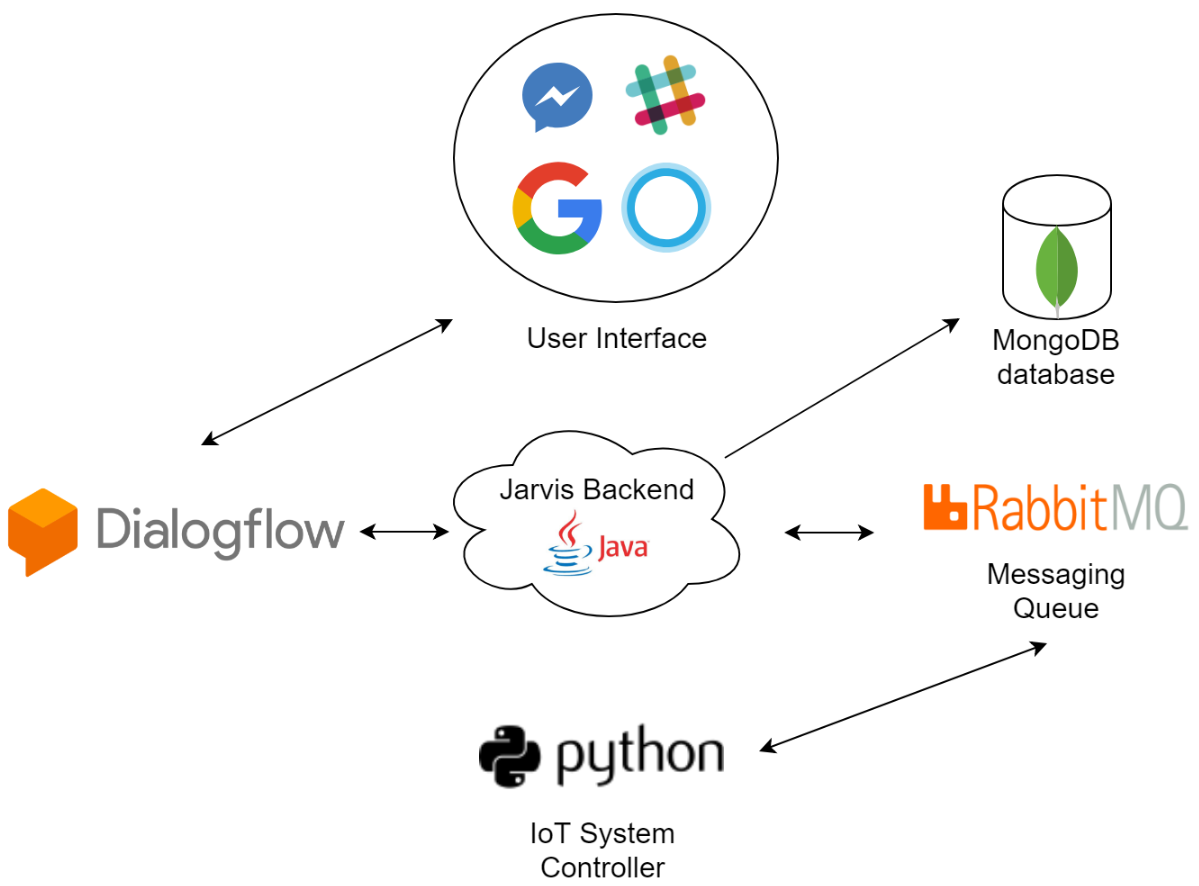
\includegraphics[width=0.5\textwidth]{figures/architecture.png}
        \caption{Jarvis overall architectural components.} \label{fig:architecture}
    \end{center}
\end{figure}

Figure~\ref{fig:architecture} presents the high level software components of Jarvis. Each of the components is explained in the following subsections.

\subsection{User Interface}
\subsection{Dialogflow Backend}
\subsection{Jarvis Backend}
\subsection{Database}
\subsection{Messaging Queue}
\subsection{IoT System Controllers}

\section{Validation}
\subsection{Simulated Scenarios}
\subsection{User Study}

\section{Conclusions and Future Work}

\begin{table}
    \caption{User Study results (task completion rate, task time and incorrect queries).}
    \centering
    \begin{tabular}{ | c | c | c | c | c | c | c | c | c | c | c | c |}
    \hline
    \multicolumn{2}{|c|}{} & \multicolumn{2}{|c|}{Time} & \multicolumn{2}{|c|}{IQ (Ast)} & \multicolumn{2}{|c|}{IQ (User)} & \multicolumn{2}{|c|}{IQ (Jvs)} & \multicolumn{2}{|c|}{IQ} \\ \hline
    Task & Done & Avg & Med & Avg & Med & Avg & Med & Avg & Med & Avg & Med \\ \hline
    
    0 (1) & 94\% & 6.4 & 6 & 0.13 & 0 & 0.25 & 0 & 0.13 & 0 & 0.5 & 0 \\ \hline
    1 (1) & 94\% & 7.1 & 7 & 0.38 & 0 & 0.5 & 0.5 & 0 & 0 & 0.5 & 0.5 \\ \hline
    2 (1) & 88\% & 10 & 10 & 0.75 & 0.5 & 0.63 & 0.5 & 0.25 & 0 & 1 & 1 \\ \hline
    3 (1) & 100\% & 20 & 19.5 & 0.13 & 0 & 0.13 & 0 & 0.75 & 1 & 1 & 1 \\ \hline
    4 (1) & 94\% & 9 & 8 & 0.25 & 0 & 0.38 & 0 & 0 & 0 & 0.63 & 0 \\ \hline
    0 (2) & 100\% & 6.4 & 6 & 0.33 & 0 & 0 & 0 & 0.33 & 0 & 0.67 & 0 \\ \hline
    1 (2) & 94\% & 7.6 & 7 & 0.11 & 0 & 0 & 0 & 0.44 & 0 & 0.56 & 0 \\ \hline
    2 (2) & 100\% & 9.9 & 10 & 0 & 0 & 0.11 & 0 & 0.78 & 1 & 0.89 & 1 \\ \hline
    3 (2) & 88\% & 19.44 & 19 & 0.33 & 0 & 0.33 & 0 & 0.22 & 0 & 0.89 & 1 \\ \hline
    4 (2) & 100\% & 8.33 & 8 & 0.33 & 0 & 0.22 & 0 & 0.22 & 0 & 0.78 & 1 \\ \hline
    \end{tabular}

    \label{table:studyresults}
\end{table}

\section{First Section}
\subsection{A Subsection Sample}
Please note that the first paragraph of a section or subsection is
not indented. The first paragraph that follows a table, figure,
equation etc. does not need an indent, either.

Subsequent paragraphs, however, are indented.

\subsubsection{Sample Heading (Third Level)} Only two levels of
headings should be numbered. Lower level headings remain unnumbered;
they are formatted as run-in headings.

\paragraph{Sample Heading (Fourth Level)}
The contribution should contain no more than four levels of
headings. Table~\ref{tab1} gives a summary of all heading levels.

\begin{table}
\caption{Table captions should be placed above the
tables.}\label{tab1}
\begin{tabular}{|l|l|l|}
\hline
Heading level &  Example & Font size and style\\
\hline
Title (centered) &  {\Large\bfseries Lecture Notes} & 14 point, bold\\
1st-level heading &  {\large\bfseries 1 Introduction} & 12 point, bold\\
2nd-level heading & {\bfseries 2.1 Printing Area} & 10 point, bold\\
3rd-level heading & {\bfseries Run-in Heading in Bold.} Text follows & 10 point, bold\\
4th-level heading & {\itshape Lowest Level Heading.} Text follows & 10 point, italic\\
\hline
\end{tabular}
\end{table}


\noindent Displayed equations are centered and set on a separate
line.
\begin{equation}
x + y = z
\end{equation}
Please try to avoid rasterized images for line-art diagrams and
schemas. Whenever possible, use vector graphics instead (see
Fig.~\ref{fig1}).

\begin{figure}
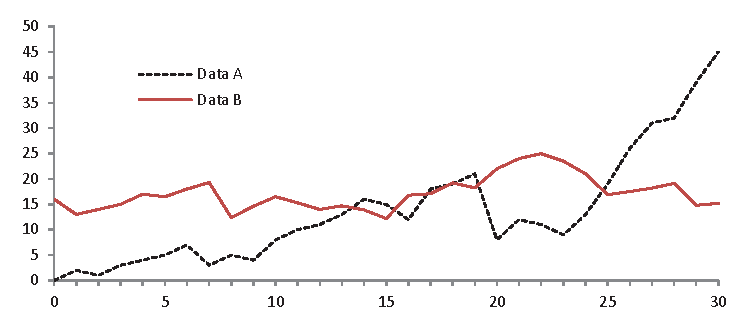
\includegraphics[width=\textwidth]{fig1.eps}
\caption{A figure caption is always placed below the illustration.
Please note that short captions are centered, while long ones are
justified by the macro package automatically.} \label{fig1}
\end{figure}

\begin{theorem}
This is a sample theorem. The run-in heading is set in bold, while
the following text appears in italics. Definitions, lemmas,
propositions, and corollaries are styled the same way.
\end{theorem}
%
% the environments 'definition', 'lemma', 'proposition', 'corollary',
% 'remark', and 'example' are defined in the LLNCS documentclass as well.
%
\begin{proof}
Proofs, examples, and remarks have the initial word in italics,
while the following text appears in normal font.
\end{proof}
% For citations of references, we prefer the use of square brackets
% and consecutive numbers. Citations using labels or the author/year
% convention are also acceptable. The following bibliography provides
% a sample reference list with entries for journal
% articles~\cite{ref_article1}, an LNCS chapter~\cite{ref_lncs1}, a
% book~\cite{ref_book1}, proceedings without editors~\cite{ref_proc1},
% and a homepage~\cite{ref_url1}. Multiple citations are grouped
% \cite{ref_article1,ref_lncs1,ref_book1},
% \cite{ref_article1,ref_book1,ref_proc1,ref_url1}.
%
% ---- Bibliography ----
%
% BibTeX users should specify bibliography style 'splncs04'.
% References will then be sorted and formatted in the correct style.
%
\bibliographystyle{splncs04}
\bibliography{mybibliography}
%
%\begin{thebibliography}{8}
% \bibitem{ref_article1}
% Author, F.: Article title. Journal \textbf{2}(5), 99--110 (2016)

% \bibitem{ref_lncs1}
% Author, F., Author, S.: Title of a proceedings paper. In: Editor,
% F., Editor, S. (eds.) CONFERENCE 2016, LNCS, vol. 9999, pp. 1--13.
% Springer, Heidelberg (2016). \doi{10.10007/1234567890}

% \bibitem{ref_book1}
% Author, F., Author, S., Author, T.: Book title. 2nd edn. Publisher,
% Location (1999)

% \bibitem{ref_proc1}
% Author, A.-B.: Contribution title. In: 9th International Proceedings
% on Proceedings, pp. 1--2. Publisher, Location (2010)

% \bibitem{ref_url1}
% LNCS Homepage, \url{http://www.springer.com/lncs}. Last accessed 4
% Oct 2017

%\end{thebibliography}
\end{document}